\chapter{State of Art of 3D Reconstruction}

\section{3D Scanning Technologies}

Many technologies exist to capture tridimensional information of the environment. The following section describes such systems and describe the basic working principle along with the pros and cons inherent to each ones. These techniques can be categorized into active and passive\cite{mada03}. In particular, three technologies are described in detail: stereoscopy, structured light and LiDAR.

\subsection{Stereoscopy}

For many years, stereoscopy remained the most popular method for 3D sensing. This system uses images taken from a pair of cameras and extracts depth information using the perspective projection: the position of objects to the sensor is relatively further apart than the objects farther from the sensor. To compute depth, features from both images are extracted and matched together, which makes it a complex and computationally demanding, so it requires fast computers or dedicated software. This system has the advantage of having a good rate of acquisition and having high resolution. Also, color information is available. However, the reconstruction algorithm rely heavy on environment characteristics, like lightning conditions, texture and non-homogeneous regions~\cite{klimentjew10}. This means that this method gives good results for edges and textured areas, but fails to get the depth information of continuous surfaces. Also, the geometric precision depends on the resolution of the images and degrades as objects are further apart.

\subsection{Structured Light}

In 2010, the availability of consumer grade depth sensors based on structured light lead to the development of consumer-grade small factor RGB-D cameras, started by Microsoft, with the \textit{Kinect} and followed by other devices, like \textit{ASUS Xtion} and \textit{Intel RealSense}. These cameras come in small form factors, are inexpensive and are capable of capturing both color and depth information at real-time rates~\cite{zollhoefer18}.

These appealing characteristics lead to a boost in the research and development in 3D reconstruction using this camera, culminating in the KinectFusion algorithm \cite{newcombe11}, capable of a fast and precise 3D reconstruction using a \textit{Kinect} RGB-D camera and commodity GPUs. This algorithm was capable of performing real-time reconstruction, using a Iterative Closest Point (ICP) for tracking the location of the device and for the registration of new RGB-D data. Nowadays, it is possible to achieve the same result using a phone equipped with a depth camera, like the \textit{Lenovo Phab 2} or \textit{ASUS Zenphone VR} and with the \textit{Google Tango} software. 

Structured light sensors work by projecting an infrared pattern onto the scene and calculate the depth via the perspective deformation of the pattern due to the different object's depth. However, this technique yields results that can be worst compared to other systems: the depth values from structured light have significant error or can be missing, specially from objects with darker colors, specular surfaces or small surfaces~\cite{shen13}. 

\subsection{LiDAR}

Light Detection and Ranging, or LiDAR, is one of the most precise and reliable ways to measure distances. It began being used shortly after the invention of Laser, in 1960, and it's valuable characteristics lead to the integration of it in the Apollo 15 mission, to serve as an altimeter to map the surface of the moon. Soon after, it was implemented in aircrafts to create high-precision and dense earth's surface models. Nowadays, its applications can be found everywhere where an accurate distance measurement is required, as for example in geology, archeology, geography and meteorology.

The success of LiDAR is related to the use of laser as its light source. Lasers are capable of emitting beams of light that are monochromatic, narrow and polarized. That is, lasers emit light in a narrow spectrum, so they can produce a single color of light, also known as monochromatic light. It improves the resilience against background light, making it possible to use even with sun light. Also, laser photons travel in a narrow beam that stays narrow even at large distances, with minimum scattering, therefore measuring the distance in a very small area in the surface. This improves the measurements near sharp transitions, where a bigger area of measurement can cause errors in the measurement. Moreover, lasers have a fast transition time, which is essential to reduce the error of the distance measurement, because it is directly influenced by the time between pulses, and a sharp transition reduces the error in the time measurement. 

LiDAR is a Time of Flight sensor. Time of flight sensors, or ToF sensors, use the speed of light to measure the distance. A scene is illuminated by a light source and the reflected light is detected back by the sensor. The time that the light has taken to travel forth and back is then measured and the depth is calculated with this time. The measurement dependes on the type of ToF system used, that is ether \textit{continuous} or \textit{pulsed}. In \textit{pulsed} systems, light is emitted in bursts with a fast shutter and the time between the emission and the reception is calculated. \textit{Continuous} systems use a modulated light source and measure the phase-shift between the outgoing and incoming wave.

This technology has some advantages comparing to both previous approaches \cite{zollhoefer18}. First, it is less computationally intensive, because the measurement is directly done by a specialized sensor. Second, it is partially independent of the lightning conditions because the light detected is emitted by the device itself. Further, it is capable of providing a dense and accurate depth values, even for continuous or irregular surfaces, unlike the stereoscopic approach. Moreover, it is much faster that any other method, capable of acquisition rates of hundreds of \si{\hertz}. However, it has some disadvantages as well. The properties of the material, like the reflectivity, color and roughness can have significant effects on the accuracy of ToF sensors. Moreover, multi-path reflections are a common problem of ToF sensors, caused by multiple reflections of the light, causing errors in the measurements. Furthermore, interference can exist if multiple ToF sensors share the same environment. However, it is possible to mitigate this effect, by either controlling the sensor such that only one is activate at a time, or by using different modulation frequencies in their illumination source.

In recent years, LiDAR scanner became a fundamental technology for industrial and robotics applications. Their small form factor and high precision are essencial for numerous applications. In general, two types of laser scanners exist: the 2D laser scanners, the one used in this work, and the 3D laser scanners. 

2D laser scanners emit a single laser beam, which is reflected by a rotating mirror to scan across a planar area. They are also the most accessible type, as their price ranges range from hundreds to tenths of thousands of Euros, depending on their characteristics. One example of this laser scanners is the SICK LMS511, shown in \cref{fig:sick-lms511}. 

\begin{figure}
    \centering
    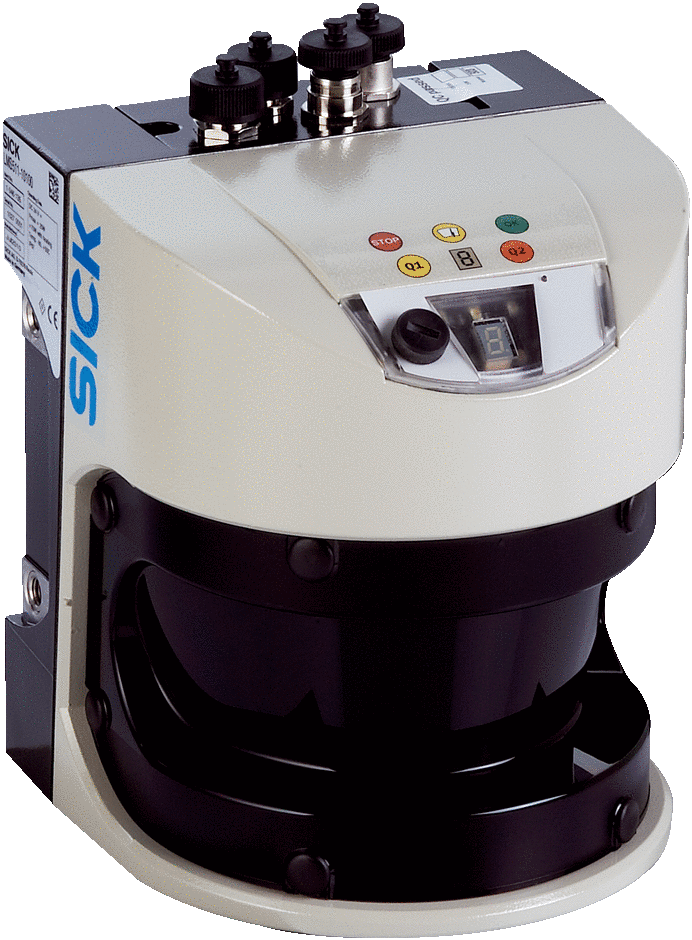
\includegraphics[width=6cm]{lms511}
    \caption{Sick LMS511 2D laser scanner.}
    \label{fig:sick-lms511}
\end{figure}

This laser scanners have a large number of applications. For example, 2D laser scanners are used in autonomous robots, to provide precise 2D mapping information of the environment, which can be user afterwards for location and navigation \cite{siritanawan17}. Compared to other technologies, like stereo vision, this one requires small processing power and yields accurate results, so their application is easy to implement and requires low processing power. 

Another widely used application is intrusion detection. The 2D laser scanner can be placed in a room or door to detect if any object enters to the space. For example, it is used to ensure the safety of workers in industrial environment, ensuring that workers do not get close to working machines. Other example is in theft prevention in museums and banks to secure specific areas against robbery or vandalism\footnote{In \url{https://www.sick.com/ag/en/industries/building-safety-and-security/c/g288283}.}.

\section{Academic Work related to 3D reconstruction}

Several scientific studies can be found concerning the research and development of 3D sensors using laser scanners, and in many studies, the 2D laser is mounted on top of a moving platform and each individual laser scan is registered on a static frame of reference, in order to create a full 3D scan. The motion of the laser scanner can be classified as continuous or discontinuous. Usually a continuous motion is used for real-time systems, like autonomous vehicles, while a discontinuous motion is used when real-time is not important, like accurate 3D reconstructions of scenes. In the following paragraphs such systems are described.

In \cite{surmann03}, a mobile robot was capable of autonomous navigation, thanks to a tilting \textit{LMS200} laser scanner, that provided a depth map of the front of the robot, with a maximum resolution of $721\times256$ points. However, a scan of $181\times256$ points took about \SI{3.4}{\second}, and scans with more points ($361$ or $721$) took double or quadruple this time, making it not suitable for real-time operation. This previous system had a limited field of view, so in \cite{zcai05} a \textit{LMS291} was mounted on a pan-tilt unit for generating a 3D point cloud with a parameterized field of view.

More recently, 3D laser scanner began being developed for real-time Simultaneous Mapping and Navigation, or SLAM, in autonomous robots. This was specially due to the \textit{DARPA Grand Challenge}, a competition to award the fastest autonomous unmanned vehicle that completed a 300 miles track. In \cite{maurelli09}, a 3D laser scanner (\cref{fig:maurelli-laser-scanner}) was developed by placing two \textit{LMS200} planar laser scanners on a rotating vertical axis, capable of generating a high-quality 3D point cloud with a \SI{360}{\degree} field of view. Several other lasers were developed by rotating the laser in a continuous motion using a turntable \cite{nemoto07}, a swinging platform \cite{yoshida11}. This sensor also became lighter, compact and modular, making it possible to integrate in multiple systems easily. One of this systems is \textit{KaRoLa} (\cref{fig:karola}), described in \cite{pfotzer14}. This laser scanner was then applied to several system, specially in search and rescue robots.

\begin{figure}[h]
    \centering
    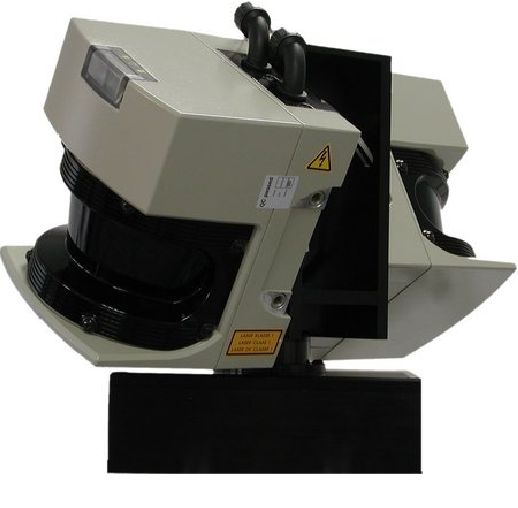
\includegraphics[width=5cm]{maurelli-laser}
    \caption{3D laser scanner developed in \cite{maurelli09}.}
    \label{fig:maurelli-laser-scanner}
\end{figure}

\begin{figure}[h]
    \centering
    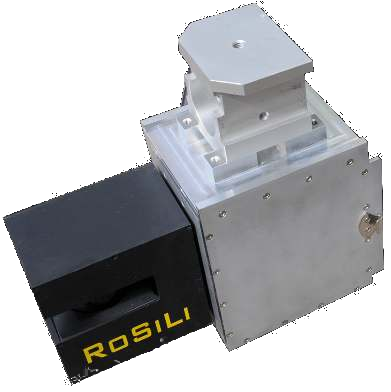
\includegraphics[width=5cm]{karola}
    \caption{The KaRoLa 3D laser scanner.}
    \label{fig:karola}
\end{figure}

The 3D laser sensors are only able to reconstruct the geometry of the scene. Some sensors are also able to measure the intensity of the reflected light, returning the reflectance value for each point. This intensity is measured, of course, in the frequency spectrum of the emitted light of the sensor, which is usually infrared (\SI{950}{\nano\meter}). To create a textured model, one or more cameras are coupled to the sensor, and both depth and color data is merged, in a process called fusion. This is specially important for areas like architecture or archeology, where color information is very important. An example of this work be seen on \cite{pdias06}, where a 3D sensor like the one described in \cite{surmann03} was paired with a camera, to generate a 3D reconstruction with color. 

These techniques were applied, for example, in cultural heritage, to model important art pieces. One of the most famous examples is the Michelangelo project \cite{levoy00}, which developed a technique to register data from a triangulation sensor and color image data to reconstruct the 3D geometry of the statue of Michelangelo's David. One of the challenges in this project was to capture the chisel marks in the surface of the status, requiring a resolution of \nicefrac{1}{4} \si{\milli\meter}, in a statue \SI{5}{\meter} tall.

\section{Comercial Solutions}

Many commercial solution exist for 3D reconstruction. In particular, two solution are presented that have similar characteristics and use-cases to this work: The Matterport and Faro Focus.

\subsection{Matterport}

\emph{Matterport} is advertized as an all-in-one solution, capable of both 3D reconstruction and capture 4K resolution images from the scene. Their target is mostly the reconstruction of indoor scenes, more specifically, from houses. The 3D model can be used to showcase the interior of the house, using both virtual reality or panoramic photography, or to make 3D measurements and automatically generate floor plans\footnote{In \url{https://matterport.com/}.}.

\emph{Matterport} offers two products: a 3D camera and a cloud service to process the raw data taken with the camera. The camera, as seen in \cref{fig:matterport-camera}, consists of two pais of sensors: two structured light sensors and a two photographic cameras\footnote{In \url{https://matterport.com/}.}. The structured light sensor has an advertized $99\%$ geometric accuracy within the \SI{4.5}{\meter} maximum range. The Photography sensor is a 4K HDR camera.

\begin{figure}[h]
    
    \centering
    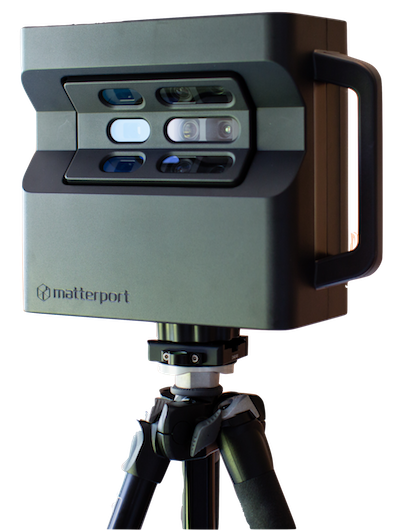
\includegraphics[width=5cm]{matterport}

    \caption{Matterport Pro2 Camera.}
    \label{fig:matterport-camera}

\end{figure}

The overall process to capture a scene is fast and easy: the 3D camera is placed on a tripod and is controlled remotely. Each acquisition takes about \SI{20}{\second} and the result is a 3D colorized mesh with 4 million vertices and a \SI{360}{\degree} panoramic photography with 134.2 MP. To scan an entire environment, an operator moves the camera to each space and make multiple new acquisitions from that space.

A set of models reconstructed from the with the Matterport solution can be found in "Matterport 3D Space Gallery"\footnote{In \url{https://matterport.com/gallery}.}. As an example, the model named "Pennsylvania Craftsman Home"\footnote{In \url{https://matterport.com/3d-space/pennsylvania-craftsman-home/}.} can be seen in \cref{fig:matterport-model}. This model represents the complete interior of an house, which look very detailed.

\begin{figure}[h]
    
    \centering
    \begin{subfigure}{\textwidth}
        \centering
        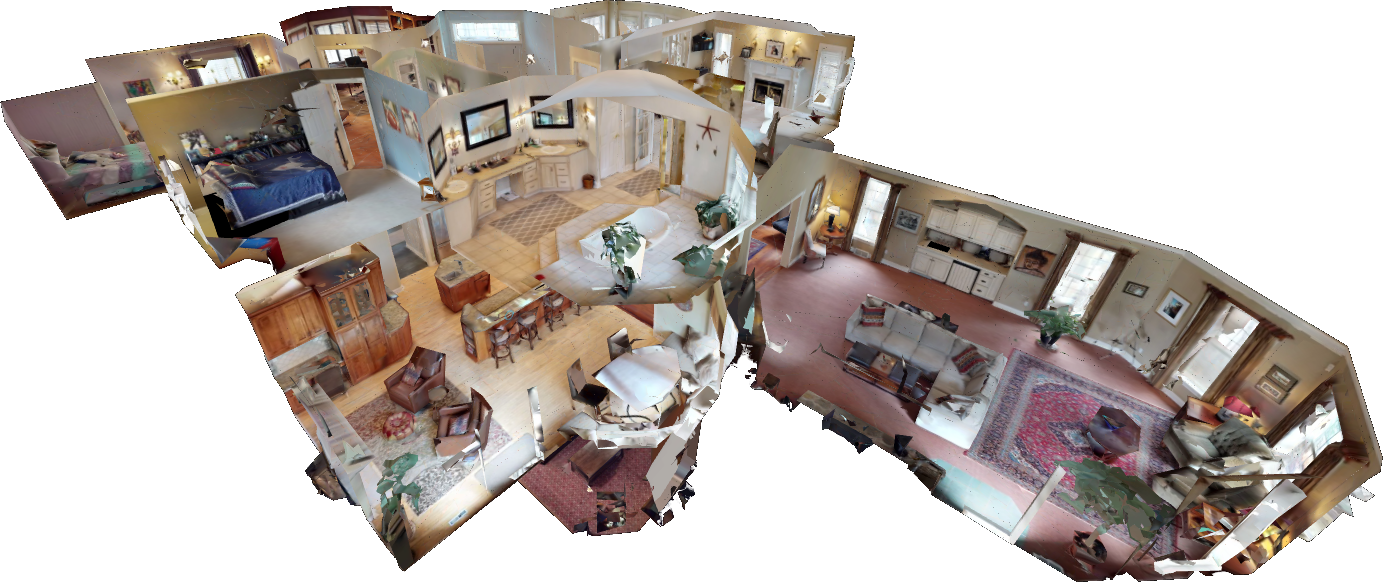
\includegraphics[width=10cm]{matterport-scan-side}
        \caption{Side view.}
    \end{subfigure}

    \begin{subfigure}{\textwidth}
        \centering
        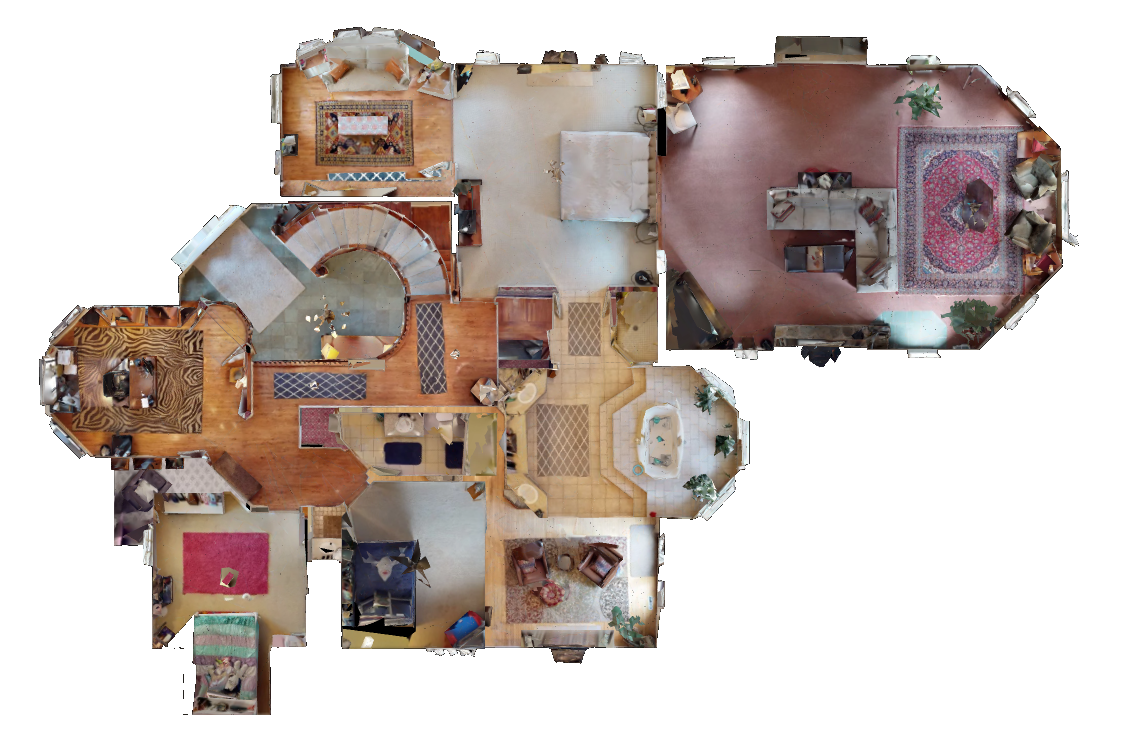
\includegraphics[width=10cm]{matterport-scan-top}
        \caption{Top view.}
    \end{subfigure}

    \caption{Matterport "Pennsylvania Craftsman Home" model.}
    \label{fig:matterport-model}
\end{figure}

\subsection{Faro Focus}

Faro Focus\footnote{In \url{https://www.faro.com/en-gb/products/construction-bim-cim/faro-focus/}.} are a series of 3D laser scanners targeted for the sectors of architecture, engineering, construction and product design. As such, this solution is capable of fast 3D reconstructions both on outside and inside environments with great accuracy. The 3D scanner (\cref{fig:faro-focus}) is design for portability and is equipped with a laser scanner with a precision of \SI{+-1}{\milli\meter} and a range of \SIrange{0.6}{350}{\meter}, and a 8 MP HDR camera.

\begin{figure}[h]
    \centering
    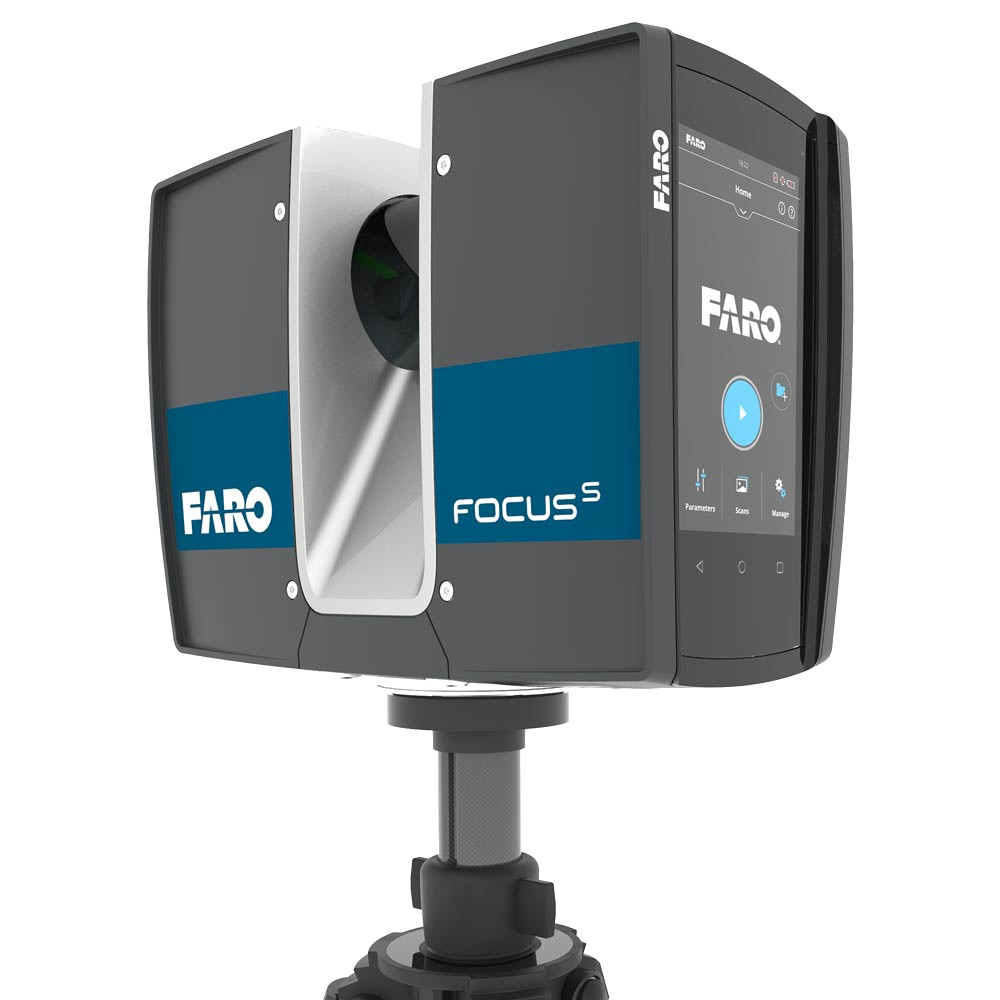
\includegraphics[width=6cm]{faro-focus}
    \caption{Faro Focus 3D laser scanner.}
    \label{fig:faro-focus}
\end{figure}

An acquisition, like in the \emph{Matterport Pro2 Camera}, is quick and easy, but does not require any remote computer, as the scanner incorporates a touch LCD screen. All the subsequent processing is done afterwards.

Faro Focus scans are very precise, as they are used for precise measurements of the reconstructed scene. As an example, a scan obtained by the Faro Focus can be seen in \cref{fig:faro-scan}\footnote{In \url{https://streambend.net/laser-scanning/}.}.

\begin{figure}[h]
    \centering
    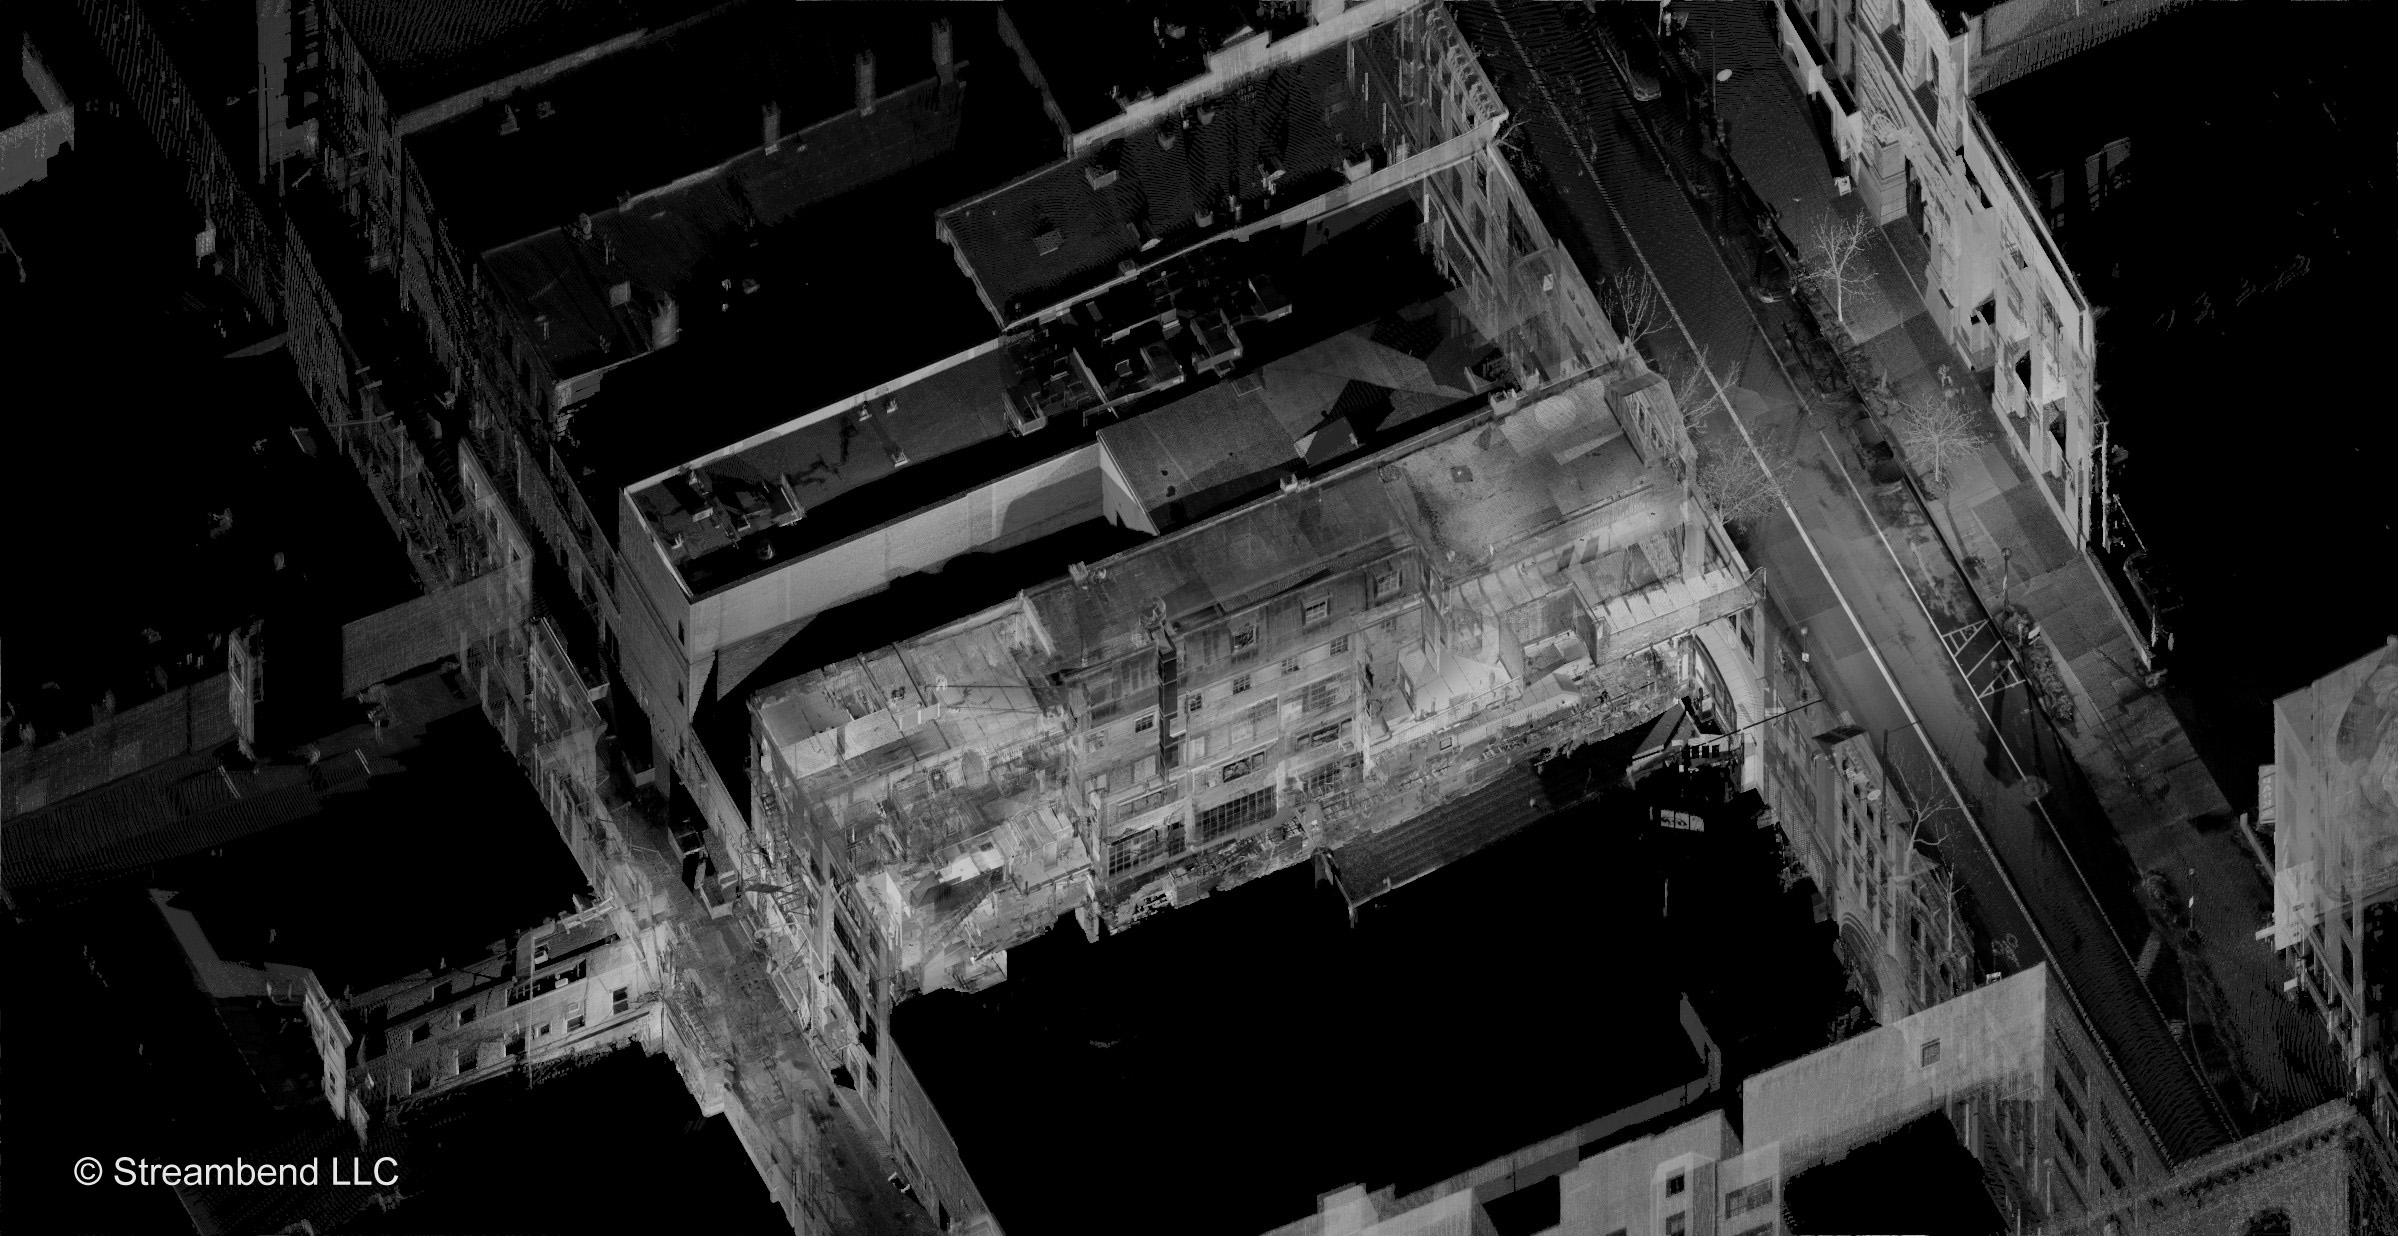
\includegraphics[width=12cm]{faro-scan}
    \caption{Faro 3D scan.}
    \label{fig:faro-scan}
    
\end{figure}
